\documentclass[12pt,a4paper]{article}
\usepackage[utf8]{inputenc}
\usepackage[german]{babel}
\usepackage[T1]{fontenc}
\usepackage{amsmath}
\usepackage{amsfonts}
\usepackage{hyperref}
\usepackage{amssymb}
\usepackage{graphicx}
\usepackage{listings}
\usepackage[left=2cm,right=2cm,top=2cm,bottom=2cm]{geometry}

%if this is changed, check if the url in the first java ref is shown correctly.
\bibliographystyle{alpha}

%configure syntag highlighting
\usepackage{listings}

%dont forget commas at end of every line!!!
\lstset{ 
language=Java,
frame=single,
%this shrinks 2 space to 1 so code can be copied from intellij without reformatting
literate={\ \ }{{\ }}1,
breaklines=true,
columns=fullflexible,
numbers=right
}

%this removes EINRÜCKUNG at text after a figure
\setlength{\parindent}{0pt}

%%this removes empty ":" after abbildung 1:
\usepackage{caption}

\newtheorem{theorem}{Definition}
\author{Frank Leuchtmann}
\title{Systematische Generierung konsistenter Mengen qualitativer
Konditionale}

% this value solves the problem overfull hbox. it defines somehow max empty space in a line.
\tolerance=950

\newcommand{\lag}{\mathcal{L}}

%%the following 2 is to define the dotl command. can this be shorter??
\newcommand\dotl{\mathrel{%
    \mathchoice{\QEQ}{\QEQ}{\QEQ}{\QEQ}%
}}
\def\QEQ{{%
    \setbox0\hbox{<}%
    \rlap{\hbox to \wd0{\hss \raisebox {0.1pt}{$\ \cdot$\hss}}}\box0
}}

\newcommand\dotll{\mathrel{%
    \mathchoice{\QEQQ}{\QEQQ}{\QEQQ}{\QEQQ}%
}}
\def\QEQQ{{%
    \setbox0\hbox{$\leqslant$}%
    \rlap{\hbox to \wd0{\hss \raisebox {1pt}{$\ \cdot$\hss}}}\box0
}}

% rdotl command
\newcommand\rdotl{\mathrel{%
    \mathchoice{\RQEQ}{\RQEQ}{\RQEQ}{\RQEQ}%
}}
\def\RQEQ{{%
    \setbox0\hbox{$\prec$}%
    \rlap{\hbox to \wd0{\hss \raisebox {0.01pt}{$\ \cdot$\hss}}}\box0
}}

\begin{document}
\maketitle
\newpage
\tableofcontents
\newpage
\section{Einleitung}
Diese Arbeit hat zum Ziel, Wissensbasen aus qualitativen Konditionalen auf eine systematische Art und Weise zu generieren. Dafür wird der in \cite{beierle19} entwickelte Algorithmus zur Berechnung aller Wissensbasen über der Signatur $\Sigma_{abc}$ implementiert. Dabei soll ergründet werden, welchen Aufwand diese Generierung mit einer steigender Anzahl der darin  enthaltenden Konditionalen verursacht. Die als Ergebnis entstandenen Wissensbasen sollen dann dazu dienen, das System InfOCF (siehe \cite{beierle17}) experimentell zu evaluieren.
\\
Der weitere Ablauf dieser Arbeit ist wie folgt: Im nächsten Kapitel werden zuerst die Grundlagen zu Konditionalen und Wissensbasen dargestellt, um die Basis für das weitere Vorgehen zu schaffen. Anschließend werden die betrachteten Koditionale in einer Normalform vollständig berechnet, dargestellt und geordnet gespeichert. Im Hauptteil dieser Arbeit wird dann ein Algorithmus aus \cite{beierle19} zur Erzeugung aller Wissensbasen über der Signatur implementiert und die Vorgehensweise dabei beschrieben. Die erhaltenen Ergebnisse werden dann in einer geeigneten Form dargestellt. Abschließend werden die gewonnenen Ergebnisse und Erkenntnisse eingeordnet.
\section{Grundlagen}
In diesem Abschnitt werden kurz die Grundlagen aufgeführt, auf denen der Hauptteil dieser Arbeit dann basiert. Die Inhalte und Darstellungen sind dabei aus den Kapiteln über Grundlagen aus \cite{beierle19} und \cite{beierle17} übernommen.
\subsection{Notation}
Zuerst wird kurz die Notation beschrieben, mit der die Konditionale im weiteren Verlauf der Arbeit dargestellt werden. Einzelne Atome, die betrachtet werden, werden mit Kleinbuchstaben wie $a, b, c,...\ $ bezeichnet. Aussagen über diese werden in Form von Großbuchstaben $A, B, C,...$ formuliert, die Gesamtheit der Sprache wird als $\lag$ bezeichnet. Die Menge der möglichen Welten, die betrachtet werden, wird mit $\Omega$ beschrieben. In einer dieser Welten $\omega \in \Omega$  hat der Ausdruck $\omega \models A$ die Bedeutung, dass $A \in \lag$ in dieser Welt gilt. Des weiteren wird $\neg A$ als $\overline{A}$ und $A \wedge B$ als $AB$ abgekürzt.
\subsection{Konditionale}
Ein Konditional ist ein Zusammenhang aus einer Vorbedingung (Antecedent) und einer Folgerung (Consequence) aus dieser Vorbedingung in der Form \glqq Wenn, A dann B\grqq . Ein qualitatives Konditional ist ein solches unter  Unsicherheit und entspricht einem Zusammenhang in der Form \glqq Wenn $A$, dann normalerweise $B$\grqq . Dargestellt wird so ein Konditional $r$ im folgenden mit dem Symbol \glqq$|$\grqq \space in der Form $r = ( \lag | \lag)$. Ein Beispiel ist $r = (B|A)$. Das dazugehörige gegenteilige Konditional lautet dann $\overline{r} = (\overline{B}|A)$.\\
Um die Akzeptanz eines unsicheren Konditionals zu bestimmen, werden sie oft im Rahmen von ordinalen Rangfunktionen nach Wolfgang Spohn betrachtet. Mehr dazu auch in diesem Text im  \autoref{sec:wissensbasen}. Vereinfacht gesagt wird ein unsicheres Konditional dann  akzeptiert, wenn es plausibler ist als das dazugehörige gegenteilige Konditional. Beispielsweise $(B|A)$ wird  dann akzeptiert, wenn $A B$ plausibler ist als $A \overline{B}$, siehe dazu auch \cite{isberner14}. \\
Das Konditional unter Unsicherheit in der Form $(B|A)$ teilt dann die Menge möglicher Welten $\Omega$ in drei Teile auf: Welten, die das Konditional bestätigen ($A B$), Welten die es falsifizieren ($A \overline{B}$) und Welten, auf die das Konditional nicht anwendbar ist, weil die Vorbedingung nicht erfüllt ist ($\overline{A}$). Die letztere Möglichkeit wird auch mit $u$ bezeichnet, was als \textit{unknown} gedeutet werden kann. Damit lässt sich das Konditional als Indikatorfunktion wie folgt darstellen:
\[
  (B|A)(\omega)=\begin{cases}
               1 \quad wenn \quad \omega \quad \models AB\\
               0 \quad wenn \quad \omega \quad \models A\overline{B}\\
               u \quad wenn \quad \omega \quad \models \overline{A}
            \end{cases}
\]

\subsection{Äquivalente und triviale Konditionale}
\label{sec:äquivalenz-konditionale}
Äquivalenz für Konditionale soll im weiteren Verlauf dadurch charakterisiert sein, dass zwei äquivalente Konditionale die Menge der möglichen Welten auf die gleiche Art und Weise unterteilen:
\begin{equation}
(B|A)\equiv (B^\prime|A^\prime) \quad gdw. \quad A\equiv A^\prime \quad und \quad AB \equiv A^\prime B^\prime
\end{equation}
Als triviale Konditionale werden solche beschrieben, die keinen Mehrwert bieten, vgl. \cite{beierle19}. Das beinhaltet sowohl sich selbst Erfüllende wie $(A \models A)$ als auch Konditionale, die einfach das Gegenteil eines anderen Konditionals in der Form $(A \models \overline{B})$ darstellen. Solche Konditionale sind bei der weiteren Betrachtung nicht von Interesse und werden daher nicht weiter beachtet.


\subsection{Ordnungsrelation für Konditionale}
\label{sec:ordnungsrelation}
In diesem Abschnitt wird eine Ordnungsrelation für Konditionale definiert, unter der Konditionale später sowohl geordnet bearbeitet als auch gespeichert werden können.
\begin{theorem}[Ordnungsrelation für Zeichen und Mengen](entnommen aus \cite{beierle19}) \ \\
Für eine Ordnungsrelation $\leqslant$ auf meiner Menge $M$ wird dessen Entsprechung für Zeichen als $\leqslant_{lex}$ notiert. Für die geordneten Mengen $S, S^\prime$ mit $S = \{e_1, ..., e_n\}$ und $S^\prime = \{e_{1}, ... , e_{n\prime}\}$ gilt:
\begin{equation}
 S \leqslant_{set} S ^\prime \quad gdw. \quad n<n^\prime, \text{ oder } n = n ^\prime \text{ und } e_1...e_n  \leqslant_{lex}  e_1^\prime ... e_{n^\prime}^\prime
\end{equation}
\label{def:sortierung-konditionale}
\end{theorem}


Bei der Signatur $\Sigma = \{ a, b, c\}$ mit der Ordnungsrelation $a \dotl b \dotl c$ ergibt sich eine Ordnungsrelation für die möglichen Mengen wie folgt: $\{a\} \dotll_{set} \{b\} \dotll_{set} \{c\} \dotll_{set} \{a,b\} \dotll_{set} \{a,c\} \dotll_{set}\{b,c\} \dotll_{set} \{a, b, c\}$. \\
Im weiteren Verlauf wird oft für die Darstellung von Konditionalen eine Notation mittels möglicher Welten verwendet. Dazu wird anstatt von Aussagevariablen die Menge der möglichen Welten aufgeführt, in denen die Aussage gilt. Für eine Aussage $F$ also in der Form $\Omega_F = \{\omega | \omega \models F \}$. Ein vollständiges Beispiel für die Aussage $A\vee\overline{B}\vee\overline{C}$ sieht dann wie folgt aus: \\
$\Omega_{a\vee\overline{b}\vee \overline{c}} = \{abc,ab\overline{c},a\overline{b}c,a\overline{b}\overline{c},\overline{a}b\overline{c},\overline{a}\overline{b}c,\overline{a}\overline{b}\overline{c}\}$ \\
Um diese Notation etwas kompakter darzustellen, wird eine Repräsentation $[[\omega]]_{\dotl}$ für eine mögliche Welt unter der Signatur $\Sigma_{abc}$ per Zahl definiert, angelehnt an deren Interpretation als Binärzahl: \\
$[[abc]]_{\dotl}  = 7,\ 
[[ab\overline{c}]]_{\dotl} = 6,\ 
[[a\overline{b}c]]_{\dotl} = 5,\ 
[[a\overline{b}\overline{c}]]_{\dotl} = 4 ,\
[[\overline{a}bc]]_{\dotl} = 3,\ 
[[\overline{a}b\overline{c}]]_{\dotl} = 2 ,\  
[[\overline{a}\overline{b}c]]_{\dotl}  = 1,\ 
[[\overline{a}\overline{b}\overline{c}]]_{\dotl} = 0 $ \\
Mit dieser Notation sieht das Beispiel von oben wie folgt aus: \\
$\Omega_{a\vee\overline{b}\vee \overline{c}} = \{ 7,6,5,4,2,1,0\}$
\begin{theorem}[Ordnungsrelation für Welten und Konditionale]\ \\(entnommen aus \cite{beierle19})\ \\
Mit einer Signatur $\Sigma$ und deren linearer Ordnung $\dotl$ sind die Ordnungen $\overset{\mathrm{\omega}}{\dotll}$ für Welten $\omega, \omega'$ und $\overset{\mathrm{c}}{\dotll}$ Konditionale $(B|A), (B'|A')$ wie folgt definiert:
\begin{equation}
\omega \overset{\mathrm{\omega}}{\dotll} \omega' \quad gdw. \quad [[\omega]]_{\dotl} \geqslant [[\omega']]_{\dotl}
\end{equation}

\begin{equation}
\label{eq:conditional-order} 
(B|A) \overset{\mathrm{c}}{\dotll} (B'| A') \quad gdw. \quad \Omega_A \overset{\mathrm{\omega}}{\dotll}_{set} \Omega_{A'} \quad oder \quad \Omega_A =  \Omega_{A'} \quad und \quad  \Omega_B \overset{\mathrm{\omega}}{\dotll}_{set} \Omega_{B'}
\end{equation}

\end{theorem}
Da sich die Unterscheidung von $\overset{\mathrm{\omega}}{\dotl}$ und $\overset{\mathrm{c}}{\dotl}$ aus dem Kontext ergibt, wird der Einfachheit halber im weiterem Verlauf $\dotl$ verwendet. \\
Mit der Signatur $\Sigma_{abc}$ ergibt sich für mögliche Welten beispielsweise $abc \dotl ab\overline{c} \dotl \overline{a}bc \dotl \overline{a} \overline{b} \overline{c}$. Ein Beispiel für die Ordnungsrelation für Konditionale ist $(abc|abc \vee ab \overline{c}) \dotl (abc | abc \vee \overline{a} \overline{b} \overline{c} )$ oder $(abc \vee \overline{a} \overline{b} \overline{c} | abc \vee ab \overline{c} \vee \overline{a} \overline{b} \overline{c}) \dotl (\overline{a} \overline{b} \overline{c} |  abc \vee ab \overline{c} \vee \overline{a} bc \vee \overline{a} \overline{b} \overline{c})$.
\subsection{Normalform für Konditionale}
Im Folgenden wird eine Normalform für Konditionale beschrieben. Das Ziel ist die klare Definition einer vollständigen und minimalen  Menge an nichttrivialen Konditionalen über einer Signatur $\Sigma$, die untereinander nicht äquivalent sind. Diese Normalform wird mit $NFC(\Sigma)$ bezeichnet.

\begin{theorem}[Normalform für Konditionale](entnommen aus \cite{beierle19})\\
Die folgende Charakterisierung beschreibt die Menge der Konditionale in Normalform über einer gegebenen Signatur $\Sigma$: \\ \\
$NFC(\Sigma) = \{(B|A)|A \subseteq \Omega_A, B \subsetneq A, B \neq \emptyset \}$ \\ \\
Für diese Menge gelten dann die folgenden drei Eigenschaften:\
 \begin{itemize}
\item{Nichttrivialität: $NFC(\Sigma)$ enthält kein triviales Konditional.}
\item{Vollständigkeit: für jedes nichttriviale Konditional in $\Sigma$ existiert ein äquivalentes Konditional in $NFC(\Sigma)$ }
\item{Minimalität: alle Konditionale in $NFC(\Sigma)$ sind paarweise nicht äquivalent.}
\end{itemize}
\end{theorem}

\subsection{Wissensbasen}
\label{sec:wissensbasen}
Eine endliche Menge $\mathcal{R} \subseteq (\lag | \lag)$ an Konditionalen wird als Wissensbasis bezeichnet. Um die Konsistenz einer Wissensbasis zu untersuchen, werden oft ordinale Rangfunktionen verwendet, welche im Folgenden kurz beschrieben werden. \\
Rangfunktionen wurden von Wolfgang Spohn entwickelt, siehe dazu auch \cite{spohn88} oder \cite{spohn12}. Eine Rangfunktion ist eine Funktion in der Form $\kappa :  \Omega \rightarrow \mathbb{N}_0 $. Mit einer Rangfuntion wird einer Welt $\omega$ aus den möglichen Welten $\Omega$ eine natürliche Zahl mittels einer Funktion $\kappa$ zugeordnet, um deren Grad an Plausibilität zu beschreiben. Mindestens eine Welt bekommt den Wert 0 zugewiesen und wird damit am meisten plausibel gekennzeichnet, weniger plausiblere Welten bekommen aufsteigend entsprechend ihrer Unplausibilität höhere Werte zugeordnet. Mittels solcher Rangfunktionen können sowohl einzelne Aussagen als auch Konditionale betrachtet werden.\\
Rangfunktion für Aussagen:
\[
 \kappa(A)=\begin{cases}
			min\{\kappa(\omega)|\omega \models A \} \quad wenn \  A \ akzeptiert \ wird \\
			\infty \quad andernfalls
            \end{cases}
\]
Rangfunktion für Konditionale:
\[
\kappa((B|A))=\begin{cases}
			\kappa(AB) - \kappa(A) \quad wenn \ \kappa(A) \neq \infty \\
			\infty \quad andernfalls
            \end{cases}
\]
Eine Aussage $A$ wird von einer Rangfunktion akzeptiert, wenn sie plausibler ist und damit einen geringeren Rang besitzt als dessen Gegenteil $\overline{A}$, z.B. $\kappa(A) < \kappa(\overline{A})$. Analaog dazu wird ein Konditional $(B|A)$ akzeptiert, wenn es einen geringeren Rang als dessen gegenteiliges Konditional $(\overline{B}|A)$ besitzt, z.B. $\kappa(AB)<\kappa(A\overline{B})$, vgl. \cite{beierle17}. Eine Wissensbasis $\mathcal{R}$ wird dann als konsistent eingeschätzt, wenn es mindestens eine Rangfunktion gibt, die alle in der Wissensbasis enthaltenen Konditionale akzeptiert.\\
Um konsistente Wissensbasen zu generieren, wird im Algorithmus GenKB der Test auf Toleranz nach \cite{goldszmidt96}S.64 verwendet. Dazu werden die Wissensbasen Schritt für Schritt um ein Konditional erweitert, wenn die Wissensbasis das Konditional toleriert. Die Toleranz ist dabei folgendermaßen definiert:
\begin{theorem}[Toleranz]
\label{def:toleranz}
Ein Konditional $(B|A)$ wird von einer Wissensbasis $\mathcal{R} = {(B_i|A_i)}$ toleriert, wenn eine Welt $\omega$ existiert die $(B|A)$ bestätigt und kein Konditional in $\mathcal{R}$ falsifiziert.
\begin{equation}
\omega \models A \wedge B \bigwedge^n_{i=1}(B_i|A_i)
\end{equation}
\end{theorem}
Ein Konditional $B|A$ nicht zu falsifizieren bedeutet in dem Zusammenhang, es entweder zu bestätigen in Form von $A \wedge B$ oder dass die Vorbedingung nicht zutrifft in Form von $\overline{A}$ also zusammengefasst $\overline{A} \vee B$. \\
Als nächstes wird die Äquivalenz von Wissensbasen betrachtet. Diese ist bei der Generierung von Wissensbasen von großer Bedeutung, um neue Wissensbasen und syntaktische Varianten bereits vorhandener Wissensbasen unterscheiden zu können. Als Maßstab für Äquivalenz zweier Wissensbasen wird im folgenden die elementweise Äquivalenz verwendet. Diese verfolgt den Grundgedanken, dass Teile einer Wissensbasis mit Teilen von anderen Wissensbasen einzeln verglichen werden können.
\begin{theorem}[Elementweise Äquivalenz von Wissensbasen] \ \\(entnommen aus \cite{beierle17b}) \ \\
$\mathcal{R}$ und $\mathcal{R'}$ sind Wissensbasen. Für diese gilt dann:
\begin{itemize}
\item{$\mathcal{R}$ ist eine elementweise äquivalente untergeordnete ($\ll_{ee}$) Wissensbasis von $\mathcal{R'}$ gdw. für jedes Konditional $(B'|A') \in \mathcal{R'}$, welches nicht selbsterfüllend ist, ein Konditional $(B|A) \in \mathcal{R}$ existiert, sodass gilt $(B|A) \equiv (B'|A')$.}
\item{$\mathcal{R}$ und $\mathcal{R'}$ sind strikt elementweise äquivalent gdw. $\mathcal{R} \ll_{ee} \mathcal{R'}$ und $\mathcal{R}' \ll_{ee}\mathcal{R}$.}
\item{$\mathcal{R}$ und $\mathcal{R'}$ sind elementweise äquivalent ($\mathcal{R} \equiv_{ee} \mathcal{R'}$) gwd. $\mathcal{R}$ und $\mathcal{R'}$ entweder inkonsistent oder strikt elementweise äquivalent sind.}
\end{itemize}
\end{theorem}
\subsection{Isomorphie und Äquivalenzklassen}
\label{sec:äquivalenz-wissensbasen}
Durch Umbenennung von Variablen ist es möglich, neue Kombinationen von Welten, Konditionalen oder Wissensbasen zu schaffen, die sich außer dieser Umbenennung nicht von den Vorhandenen unterscheiden. Dieses Verhalten wird als Isomorphismus beschrieben. Die jeweils zusammengehörige Gruppe an durch diesen Isomorphismus entstandenen Dingen wird dann als Äquivalenzklasse bezeichnet.\\
Beispielsweise enthält die Signatur $\Sigma_{abc}$ die mögliche Kombination $\overline{a}bc$. Wenn jetzt $a$ in $b$ und $b$ in $a$ umbenannt wird, entsteht der Isomorphismus $a\overline{b}c$. Analog kann durch Umbenennung von $a$ und $c$ daraus $ab\overline{c}$ entstehen. Alle drei bilden zusammen eine Äquivalenzklasse. Entsprechend ergibt sich die folgende Definition.
\begin{theorem}[Isomorphismus](entnommen aus \cite{beierle19}) \ \\
$X, X'$ sind Welten, Aussagen, Wissensbasen oder Mengen dieser Dinge. $X$ und $X'$ sind dann isomorph $(X \simeq X')$, wenn eine Umbenennung in der Form $\rho(X) = X'$ existiert.
\end{theorem}
Für die Signatur $\Sigma_{abc}$ ergeben sich dann die folgenden vier Äquivalenzklassen: \\
$[\Omega_{\Sigma abc}]_{/\simeq}=\{[abc]$, $[ab\overline{c}, a\overline{b}c\, \overline{a}bc], [a\overline{b}\overline{c}, \overline{a\\}b\overline{c}, \overline{a}\overline{b}c], [\overline{a}\overline{b}\overline{c}]\}$ \\
Die Menge der Äquivalenzklassen in einer Menge $M$ mit dem Element $m \in M$ wird im Folgenden mit $[M]_{/\equiv}$ und die konkrete Äquivalenzklasse welche $m$ enthält mit $[m]_\equiv$ notiert.\\
Mit Berücksichtigung von Äquivalenzklassen und der Ordnung $\dotl$ aus \autoref{sec:ordnungsrelation} wird in der nächsten Definition eine Ordnungsrelation konstruiert, die diese Äquivalenzen mit einbezieht.


\begin{theorem}[$cNFC(\Sigma)$ $und$ $Ordnungsrelation$ $\rdotl$](entnommen aus \cite{beierle19}) \ \\
Gegeben sei eine Signatur $\Sigma$ mit der linearen Ordnung $\dotl$. Dann sind $[NFC(\Sigma)]_{/ \simeq}=\{[r_1]_\simeq,...,[r_m]_\simeq\}$ die Äquivalenzklassen von $NFC(\Sigma)$ induziert durch Isomorphismus. Für jedes $i \in \{1, ..., m\}$ ist dann das Konditional $r_i$ das minimale Element in $[r_i]_\simeq$ im Sinne von $\dotl$ ist und $r_1\dotl...\dotl r_m$.
\begin{itemize}
\item{Die kanonischen Konditionale in Normalform über $\Sigma$ sind $cNFC(\Sigma) = \{r_1, ..., r_m \}$.}
\item{Die kanonische Ordnung auf $NFC(\Sigma)$ ($\rdotl)$ ist durch folgendes Schema gegeben: \\
$r_1\rdotl ... \rdotl r_m \rdotl[r_1]_\simeq \setminus \{r_1\} \rdotl ... \rdotl [r_m]_\simeq \setminus \{r_m\}$ \\ 
mit $r \rdotl r'$ gdw. $r\dotl r'$ für alle $i \in \{1, ..., m\}$ und alle $r, r' \in [r_i]_\simeq \setminus \{r_i\}$.}
\end{itemize}
\label{def:sortierung-nfc}
\end{theorem}


\section{Strukturierung des Vorgehens}
Das Ziel des weiteren Vorgehens ist es, den Algorithmus GenKB aus \cite{beierle19} praktisch umzusetzen und möglichst viele Wissensbasen auf Basis der Signatur $\Sigma=\{a,b,c\}$ zu generieren. Da aufgrund der Menge der möglichen Konditionale das Ziel nicht auch nur Ansatzweise vollständig bearbeitet werden kann, wird oft auch auch die Signatur $\Sigma=\{a,b\}$ betrachtet. Mit dieser reduzierten Signatur ist es möglich, aufgrund der deutlich geringeren Menge an Konditionalen alle möglichen Wissensbasen zu generieren. Damit lässt sich am kleineren Beispiel prüfen, ob die grundsätzliche Vorgehensweise korrekt ist und letztendlich die Aufgabenstellung vollständig lösen könnte. \\
Die Aufgabenstellung wird dafür in zwei Teile gegliedert. Im ersten Teil werden die Konditionale in Normalform basierend auf der Signatur $\Sigma=\{a,b,c\}$ berechnet und somit die Menge aller Konditionale $NFC$  berechnet. Anschließend werden auf dieser Menge an Konditionalen die Äquivalenzklassen Untersucht und damit die Menge der kanonischen Konditionale $cNFC$ sowie die einzelnen Äquivalenzklassen berechnet. Dabei werden die Konditionale auch nach der Ordnunggsrelation $\rdotl$ sortiert. Dazu werden im ersten Teil die Konditionale auf der Klasse \textit{WConditional} (W für Worlds) bearbeitet. Diese Repräsentation spiegelt die Darstellung von Konditionalen in Normalformen in \cite{beierle19} wieder. Diese Darstellung ist außerdem dafür optimiert, die in \cite{beierle19} dargestellte Ordnung im Sinne von $\rdotl$ zu repräsentieren und ermöglicht so die Sortierung der Konditionale und damit die Betrachtung von Äquivalenz. \\
Im zweiten Teil dieser Arbeit findet dann die eigentliche Generierung der Wissensbasen statt. Dazu werden die Konditionale ausgehend von Objekten der Klasse \textit{WConditional} in Objekte der Klasse \textit{PConditional} (P für Propositional logic) übersetzt. Diese Klasse ist dann für die Arbeit mit Aussagenlogik optimiert und ermöglicht so die Prüfung von Konsistenz und damit die Anwendung für den Algorithmus GenKB.




\section{Berechnung und Sortierung der Konditionale}




\subsection{NFC Creator}
In diesem Abschnitt wird beschrieben, wie das erste Teilproblem, die Berechnung der Konditionale und deren Gruppierung in Äquivalenzklassen, gelöst wird. Dazu wurde ein Programm namens NFC Creator erstellt. Dieses Programm wird dafür genutzt, um die Konditionale zu erzeugen, aus denen dann die Wissensbasen generiert werden. Der NFC Creator hat zusätzlich eine eigene grafische Oberfläche namens NFC Viewer, ein Screenshot davon ist in \autoref{pic:nfc-viewer} zu sehen. Damit können die erstellten Konditionale betrachtet und gespeichert werden. Es ist dadurch auch möglich, Teilergebnisse aus dem Erstellungsprozess der Konditionale anzuzeigen, um den Vorgang besser nachvollziehen zu können. \\
\begin{figure}
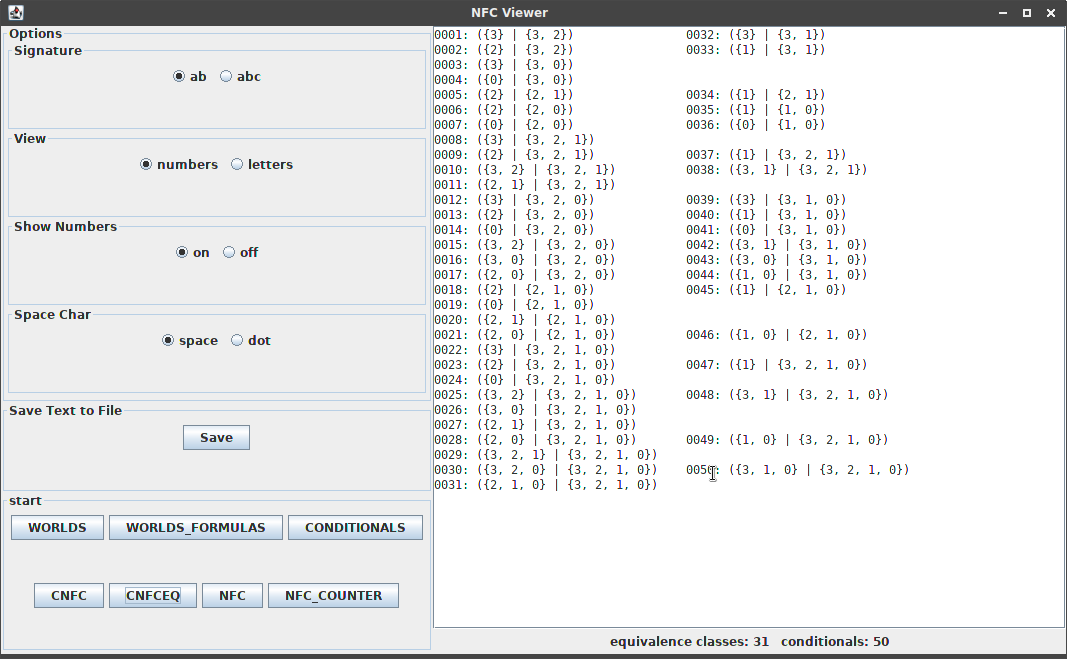
\includegraphics[width=0.8\linewidth]{bilder/nfc-viewer.png}

\caption{Screenshot NFC Viewer mit Ansicht analog zu Tabelle 1 aus \cite{beierle19}}
\label{pic:nfc-viewer}
\end{figure}
Das Programm ist intern nach dem Model-View-Controller Schema aufgebaut. Die Beschreibung hier im Text fokussiert sich dabei auf das fachliche Modell dahinter und an einigen Stellen auf die Bedienung und Präsentation der grafischen Oberfläche. Das Fachliche Modell wird zentral in der Klasse NFCCreator zusammengefasst, hier werden die einzelnen Teilschritte Koordiniert. Da die Aufgabe des NFCCreator nicht besonders rechenintesiv ist, besteht das Programm nur aus einem einzigen Thread. Die wichtigen Elemente des fachlichen Modells werden in den nächsten Unterabschnitten beschrieben. Die Logik der GUI und des Controllers werde nicht beschrieben, da sie für das fachliche Thema uninteressant sind. \\
Der grundsätzliche Aufbau der GUI besteht aus zwei Teilen. Links befinden sich im oberen Bereich die Auswahl der Optionen, darunter unter Start befinden sich die Buttons mit den möglichen Aktionen. Auf der rechten Seite befindet sich ein Textfenster, was das Ergebnis der gewählten Optionen und Aktion zeigt sowie darunter einer kurzen Beschreibung des Inhalts des Textfelds. \\
Im Folgenden werden die Optionen im Menü erklärt. Die Auswahl der Signature bietet selbsterklärend die Möglichkeiten $ab$ und $abc$. Die Option View stellt ein, ob eine mögliche Welt in Buchstabenform oder als Repräsentation als Zahl erfolgen soll. Beispielsweise wird mit Signatur $ab$ die mögliche Welt $a \overline{b}$ entweder als $a!b$ oder als 2 dargestellt. Mit der Option ShowNumbers lässt sich einstellen, ob die angezeigten Objekte, beispielsweise Konditionale, mit nummeriert dargestellt werden sollen oder nicht. Die letzte Option SpaceChar stellt einen Platzhalter für mehrere auf einer Zeile angezeigte Objekte ein. Im Screenshot ist die Option auf Space. Wird Dot aktiviert, werden zeilenweise kleine Punkte angezeigt, damit der Betrachter die Zeilen am Bildschirm etwas leichter verfolgen kann als auf rein weißem Untergrund. Das untenliegende Feld bietet mit dem Save Button die Möglichkeit, den Inhalt des Textfensters zu speichern.

\subsection{Die Klasse WorldsList}
\label{sec:worldslist}
Die Bezeichung der möglichen Welten wurde in \autoref{sec:ordnungsrelation} schon gezeigt, an diesem Punkt setzt die Betrachtung hier an. Wie beschrieben, lassen sich aussagenlogische Ausdrücke als Menge der damit enthaltenden Welten darstellen. Eine solche Menge möglicher Welten wird mit einem Objekt der Klasse WorldsList dargetellt. Objekte der Klasse WorldsList repräsentieren später in den Konditionalen dann Antecedent und Consequence. Die Gesamtheit aller solcher möglicher Mengen einer Signatur bestimmt dann die Menge der möglichen Konditionale, die über einer Signatur gebildet werden können. Der Algorithmus, der alle Mengen aus den möglichen Welten einer Signatur berechnet, ist in \autoref{code:subsets} dargestellt. Als Input wird die Liste möglicher Welten der Signatur verwendet, der Output ist eine Liste aller Teilmengen des Inputs. \\
Für die Signatur $\Sigma = \{abc\}$ ergeben sich damit 255 verschiedene Mengen von Welten. (Vergleich: für $\Sigma=\{ab\}$ sind es 15) Diese können mit dem NFC-Viewer mit dem Button "WORLDS" \space geordnet betrachtet werden. Dargestellt im Programm werden diese Mengen jeweils durch eine Instanz der Klasse WorldsList, von der ein vereinfachtes Diagramm in \ref{pic:worldslist} gezeigt ist. 


\begin{figure}
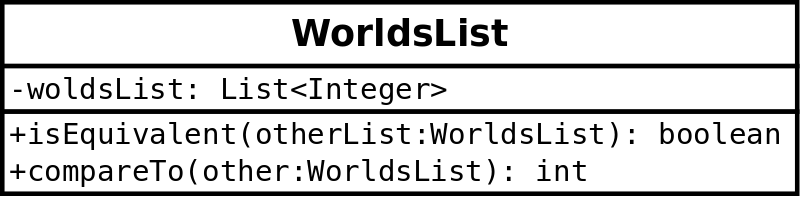
\includegraphics[width=0.45\linewidth]{bilder/worldslist.png}
\caption{WorldsList}
\label{pic:worldslist}
\end{figure}


Das wichtigste Attribut derKlasse WorldsList ist die Liste an möglichen Welten, dargestellt durch eine List<Integer>. Die Klasse WorldsList selbst implementiert weiterhin das bekannte Java Interface  \textit{Comparable} (siehe dazu auch \cite{oracle2019}) und kann damit Objekte erzeugen, die standardisiert untereinander sortiert werden können. Dazu besitzt die Klasse die Methode \textit{compareTo(Object o)} zur Sortierung gemäß Definition \ref{def:sortierung-konditionale}. Dazu vergleicht das Objekt sich selbst mit einem Anderen (dieser Klasse) und gibt als Rückgabewert entweder -1 zurück, wenn das aktuelle  Objekt (\textit{this}) kleiner als das übergebene ist, 0 wenn sie gleich sind und 1 wenn das aktuelle Objekt größer als das übergebene Objekt ist. Die Implementierung der \textit{compateTo(Object o)} Methode ist in \autoref{code:compare-worldslist} dargestellt. Das Interface  \textit{Comparable} und \textit{compareTo(Object o)} wird ähnlich wie hier später auch in anderen Klassen verwendet um die Sortierung von Objekten zu ermöglichen.



\begin{figure}
\begin{lstlisting}
private List<WorldsList> createSubSetList(List<Integer> inputList){
    List<WorldsList> subSetList = new ArrayList<>();
    for (Integer world : inputList) {
        for (ListIterator<WorldsList> setsIterator = subSetList.listIterator(); setsIterator.hasNext(); ) {
            WorldsList newWorld = new WorldsList();
            newWorld.addList(setsIterator.next().getWorldsList());
            newWorld.addInt(world);
            setsIterator.add(newWorld);
        }
        WorldsList otherWorld = new WorldsList();
        otherWorld.addInt(world);
        subSetList.add(otherWorld);
    }
    return subSetList;
}
\end{lstlisting}
\caption{Algorithmus zur Erstellung aller Teilmengen einer Liste möglicher Welten}
\label{code:subsets}
\end{figure}



\begin{figure}
\begin{lstlisting}
public int compareTo(Object o) {
    WorldsList otherWorld = (WorldsList) o;
    if (worldsList.size() < otherWorld.getWorldsList().size())
        return -1;
    if (worldsList.size() > otherWorld.getWorldsList().size())
        return 1;
          
      for (int i = 0; i < worldsList.size(); i++) {
        if (worldsList.get(i) > otherWorld.getWorldsList().get(i))
            return -1;
        if (worldsList.get(i) < otherWorld.getWorldsList().get(i))
            return 1;
    }
    return 0;
}
\end{lstlisting}
\caption{Implementierung compareTo(Object o) der Klasse WorldsList}
\label{code:compare-worldslist}
\end{figure}


Weiterhin existiert die Methode \textit{createRenamings()}, welche eine wichtige Rolle für das spätere Finden von äquivalenten Wissensbasen besitzt. Äquivalente Wissensbasen wurden bereits in  \autoref{sec:äquivalenz-wissensbasen} beschrieben. Wie oben erwähnt, entsteht diese Äquivalenz aus einer möglichen Umbenennung von Variablen. So eine Umbenennung ist jeweils nur innerhalb einer Gruppe von Konditionalen möglich, diese Gruppe wird dann Äquivalenzklasse genannt. Entsprechend ergibt sich aus der Menge der möglichen Umbenennungen die Menge an Konditionalen innerhalb einer Äquivalenzklasse. Mit Signatur $\Sigma=\{ab\}$ existiert eine einzige mögliche Umbenennung, nämlich wenn $a$ in $b$ und $b$ in $a$ umbenannt wird. Mit der Signatur $\Sigma=\{abc\}$ existieren drei mögliche Umbenennungen durch den Tausch der folgenden Paare an Variablen: $a-b$, $a-c$ und $b-c$. Die Methode \textit{createRenamings()} gibt nun in Abhängigkeit von der gewählten Signatur alle möglichen Umbenennungen einer WorldsList als neue List<WorldsList> in der oben genannten Reihenfolge wieder. Bei nur einer existierenden Umbenennung mit $\Sigma=\{ab\}$ stellt sich die Frage nach der Reihenfolge offensichtlich nicht, bei $\Sigma=\{abc\}$ spielt die immer gleiche Reihenfolge später dann eine Rolle.


\begin{figure}
\begin{lstlisting}
List<Integer> intList = new ArrayList<>(worldsList.size());
for (int world : worldsList) {
    switch (world) {
        case 0:
            intList.add(0);
              break;
        case 1:
            intList.add(1);
              break;
        case 2:
            intList.add(4);
            break;
        case 3:
            intList.add(5);
            break;
        case 4:
            intList.add(2);
            break;
         case 5:
            intList.add(3);
            break;
        case 6:
            intList.add(6);
            break;
        case 7:
            intList.add(7);
            break;
        default:
            throw new RuntimeException("Finding equivalent WorldsList failed!");
    }
}
WorldsList worldsList = new WorldsList();
worldsList.addList(intList);
renamingsList.add(worldsList);
\end{lstlisting}
\caption{Beispiel der Implementierung einer Umbenennung in der Methode \textit{createRenamings} für die Umbenennung $a-b$ in der Klasse WorldsList}
\label{code:renaming}
\end{figure}


Im Folgenden wird nun die Methode \textit{createRenamings()} der Klasse WorlsList genauer erklärt. Das Wesen einer Umbenennung einer WorldsList ist es, dass sich die enthaltene Liste der Welten ändert. Es wird für eine Umbenennung also ein neues Objekt der Klasse WorldsList mit einer neuen List<Integer> Liste der möglichen Welten erstellt. Bei jeder möglichen Umbenennung ändern sich die enthaltenen möglichen Welten auf die selbe Weise, entsprechend wird die ursprüngliche List<Integer> Liste der Welten nach einem charakteristischem Schema "übersetzt". So ein Schema existiert für jede mögliche Umbenennung, entsprechend gibt es für $\Sigma=\{ab\}$ eines und für $\Sigma=\{abc\}$ drei davon. Da der Code für all die Umbenennungen umfangreich ist und viel Platz benötigt wird hier nicht die ganze Methode \textit{createRenamings} dargestellt. In \ref{code:renaming} ist beispielhaft die Umbenennung $a-b$ mit der Signatur $\Sigma\{acb\}$ gezeigt. In Zeile 1 wird die neue List<Integer> erstellt, in die die übersetzten Werte mit einer Switch Anweisung eingetragen werden. Man sieht, dass sich  Welt 0 ($!b!b!c$) und Welt 7 ($abc$) offensichtlich nicht ändern, eine Umbenennung hat hier grundsätzlich keinen Einfluss. Welt 1($!a!bc$) und Welt 6 ($ab!c$) ändern sich bei der Umbenennung $a-b$ offensichtlich auch nicht. Die andern Welten werden durch die Umbenennung durch ein Äquivalent ersetzt. In Zeile 32 und 33 wird die neue WorldsList dann erstellt und in Zeile 34 wird sie in die List<WorldsList> der Umbenennungen eingefügt.  Für die Umbenennungen $a-c$ und $b-c$ existiert jeweils ebenfalls ein entsprechendes Stück Code und so werden alle 3 Umbenennungen realisiert. Mit $ \Sigma=\{ab\}$ existiert nur eine Umbenennung und es wird einfach Welt 1 und 2 vertauscht.




\subsection{Die Klasse WConditional}

\begin{figure}
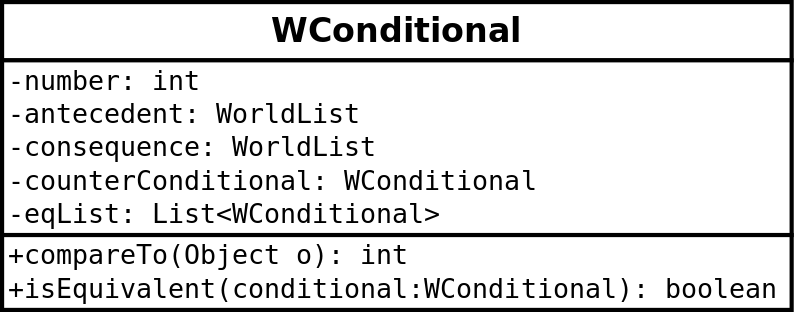
\includegraphics[width=0.55\linewidth]{bilder/wconditional.png}
\caption{WConditional}
\label{pic:wconditional}
\end{figure}

Die Klasse WConditional bildet die Basis für die Berechnung der Konditionale aus einer vorgegebenen Signatur. Der Fokus der Klasse liegt dabei auf der Generierung, Ordnung und Betrachtung der Äquivalenz der Konditionale. Ein vereinfachtes Diagramm der Klasse ist in \autoref{pic:wconditional} zu sehen. Attribute der Klasse sind zum einen Antecedent und Consequence in Form eines WordsList Objekts. Weiterhin CounterConditional ebenfalls als Objekt der Klasse WConditional und einer Liste von äquivalenten Konditionalen als Objekte von WConditional.\\
Außerdem ist die Nummer des Konditionals gemäß der Ordnung $\rdotl$ gemäß Definition \ref{def:sortierung-nfc} als int Variable enthalten.



\begin{figure}
\begin{lstlisting}
public int compareTo(Object o) {
    WConditional otherConditional = (WConditional) o;
    if (this.antecedent.compareTo(otherConditional.getAntecedent()) != 0)
        return this.antecedent.compareTo(otherConditional.getAntecedent());
    else return this.consequence.compareTo(otherConditional.getConsequence());
}
\end{lstlisting}
\caption{Implementierung compareTo(Object o) der Klasse WConditional}
\label{code:compare-wconditonal}
\end{figure}


Die Klasse WConditional ist ebenfalls sortierbar mit dem Interface \textit{Comparable}, die Implementierung der \textit{compareTo(Object 0)} Methode ist in \autoref{code:compare-wconditonal} gezeigt. Die Implementierung entspricht damit genau der Sortierung nach $\overset{\mathrm{c}}{\dotll}$ wie in \autoref{eq:conditional-order} beschrieben.



\begin{figure}
\begin{lstlisting}
public boolean equals(Object o) {
    if (!(o instanceof WConditional))
        return false;
    else {
        WConditional otherConditional = (WConditional) o;
        boolean leftEquals = otherConditional.getConsequence().equals(consequence);
        boolean rightEquals = otherConditional.getAntecedent().equals(antecedent);
        return leftEquals && rightEquals;
    }
}
\end{lstlisting}
\caption{Implementierung \textit{equals(Object 0)} der Klasse WConditonal}
\label{code:equals-wconditonal}
\end{figure}


Eine sehr wichtige Methode der Klasse WConditonal ist die Überschreibung der \textit{equals(Object o)} Methode. Diese ist in \autoref{code:equals-wconditonal} zu sehen. Sie liefert dann true zurück, wenn die WorldsList Objekte beider WConditonals dieselben sind. Zwei solche Instanzen von WorldsList sind genau dann die selben, wenn sie die selbe Menge an möglichen Welten enthalten. Intern wird hier einfach die beiden List<Integer> worldsList miteinander verglichen. Die Methode \textit{createEquivalentConditonals(..)} ist unter \autoref{sec:counter-conditonals} genauer beschrieben.


\subsection{Berechnung aller Konditionale}




In \autoref{sec:worldslist} wurden bereits die 255 verschiedenen Kombinationen der möglichen Welten unter Signatur $\Sigma=\{a,b,c\}$ gebildet. In diesem Abschnitt wird gezigt, wie aus diesen Kombinationen alle möglichen Konditionale in Normalform als Objekte der gerade beschriebenen Klasse WConditional generiert werden. \\
Als Input dafür wird die Liste an WorldsLists aus \autoref{sec:worldslist} mit ihren 255 Elementen verwendet. Der Algorithmus zur Generierung aller möglichen Kombinationen daraus ist in \autoref{code:create-conditionals} zu sehen. Der Output der Methode ist eine Liste aller möglichen Konditionale in Normalform. \\
Dazu iteriert der Algorithmus in Zeile 4 über alle möglichen Mengen von Welten, diese bilden dann jeweils den Antecedent der Konditionale. Für jede dieser Iterationen werden im Zeile 8 alle echten Teilmengen des Antecedent gebildet, woraus sie die Consequent bildet. Aus Antecedetnt und Consequent wird dann jeweils ein Konditional gebildet. Zum Schluss werden die Konditionale in Zeile 15 nach der Ordnung $\dotl$ in \autoref{eq:conditional-order} sortiert. Bei Ausführung mit der Signatur $\Sigma=\{ab\}$ ergeben sich die 50 Konditionale wie in der Orginalquelle \cite{beierle19} dargestellt. Bei Ausführung mit $\Sigma=\{abc\}$ entstehen 6050 Kontitionale, die die Ausgangsbasis für die Generierung der Wissensbasen bilden. Die Konditionale können in der GUI des Programms NFC Creator mit dem Button CONDITIONALS betrachtet werden.

\begin{figure}
\begin{lstlisting}
private List<WConditional> createBasicConditionalList(List<WorldsList> worldsList) {
    List<WConditional> basicConditionalList = new ArrayList<>();
    for (WorldsList currentWorld : worldsList) {
        List<WConditional> currentConditionalList = new ArrayList<>();
        List<WorldsList> allSubSetsOfCurrentWorld = createSubSetList(currentWorld.getWorldsList());
        for (WorldsList currentSubSworld : allSubSetsOfCurrentWorld) {
            //only add real subsets not the set itself
            if (!currentSubWorld.equals(currentWorld))
                currentConditionalList.add(new WConditional(currentSubWorld, currentWorld));
        }
        basicConditionalList.addAll(currentConditionalList);
    }
    Collections.sort(basicConditionalList);
  return basicConditionalList; }
\end{lstlisting}
\caption{Algorithmus zur Generierung aller Konditionale aus einer gegebenen Liste Möglicher Kombinationen von Welten}
\label{code:create-conditionals}
\end{figure} 


\subsection{Äquivalenzklassen und Sortierung der Konditionale}

\label{sec:equivalence}

Im Abschnitt zuvor wurden die Konditionale nach der Ordnung $\dotl$ abgespeichert. In diesem Abschnitt wird beschrieben wie die Sortierung nach der Ordnung $\rdotl$, welche unter unter \autoref{def:sortierung-nfc} gezeigt wurde, für die Klasse WConditional implementiert ist. Dazu müssen die Konditionale zunächst in Äquivalenzklassen wie in \autoref{sec:äquivalenz-konditionale} gezeigt gruppiert und dann untereinander sortiert weden. \\
Um zu prüfen, ob ein Objekt der Klasse WContitional äquivalent zu einem Anderen ist, besitzt die Klasse die Methode \textit{isEquivalent(WConditonal otherConditional)}, die in \autoref{code:test-equivalence} dargestellt ist. In diesem Algorhitmus wird geprüft, ob sich in der Liste der äquivalenten Konditionale (getBasicEquivalents()) ein äquivalentes Konditional zum übergebenen Konditional (otherConditional) existiert und entsprechend true oder false zurückgegeben. Die Methode \textit{getBasicEquivalents()} gibt eine Liste and WConditional Objekten zurück, mit der Methode createBasicEquivalents() erstellt wird. Diese Liste äquivalenter Konditionale beinhaltet dabei jedoch \textit{neu erstellte} Objekte äquivalenter Konditionale, nicht die \textit{tatsächlichen} Objekte der Äquivalenten Konditionale. Die tatsächlichen Objekte können erst nachher gruppiert werden. Ursprünglich sollte die Methode zum testen der Äquivalenz diese Liste der Äquivalenten Konditionale bei jedem Test erstellen, allerdings ist die Generierung sehr Zeitaufwendig und die Äquivalenz wird im gesamten Ablauf sehr oft geprüft (mit $\Sigma=\{abc \}$ 1550 mal, mit $\Sigma=\{abc\}$ dagegen schon 16.784.250 mal), sodass die Methode \textit{getBasicEquivalents()} sicherstellt, dass die Liste Äquivalenter Konditionale nur einmal erzeugt wird. Die Zeiteinsparung dadurch ist deutlich spürbar.\\ 
Die Methode zur Erstellung der Liste der äquivalenten Konditionale ist in \autoref{code:create-equivalents} abgebildet. In Zeile 3 und 4 wird für Antecedent und Consequence jeweils eine Liste der Umbenennungen erstellt, was in \autoref{sec:worldslist} bereits erklärt wurde. Dieser Umbenennungen werden in Zeile 6 iteriert und für alle Paare von Antecedent und Consequence wird ein neues Konditional als mögliche Umbenennung gespeichert, wenn die Umbenennung wirklich verschieden vom Ausgangskonditional ist. Wenn ein Konditional keine äquivalenten Konditionale besitzt, sind die Umbenennungen an dieser Stelle sonst gleich wie das Ursprungskonditional. Beispielsweise würden Umbenennungen des Konditionals $(ab|!a!b,ab)$ sonst immer wieder das gleiche Konditional entstehen lassen.


\begin{figure}
\begin{lstlisting}
public boolean isEquivalent(WConditional otherConditional) {
    for (WConditional eqConditional : getBasicEqList())
        if (otherConditional.equals(eqConditional))
            return true;
    return false;
}
\end{lstlisting}
\caption{Algorithmus zur Prüfung der Äquivalenz der Klasse WConditional}
\label{code:test-equivalence}
\end{figure} 


Der Ablauf der Erstellung der Liste der Konditionale NFC ist dann wie folgt: Der NFC Creator beginnt dann durch die Liste der Konditionale zu iterieren und erstellt für jedes gefundene Konditional eine eigene Liste. Für jedes dieser Konditionale wird dann mit der \textit{isEquivalent(..)} Methode der Rest der urprünglichen Liste auf Äquivalenz überprüft und die \textit{tatsächlichen} Objekte der äquivalenten Konditionale werden in die Liste eingefügt und aus der ursprünglichen Liste entfernt. Die neue Liste wird dann jeweils mit der compare(..) Methode sortiert. Dadurch entsteht eine Liste von Listen von den tatsächlichen Objekten der äquivalenten Konditionale. Diese Darstellung enspricht dann der Darstellung der Konditionale in \cite{beierle19}. Mit dem NFC Viewer kann diese Ansicht mit dem Botton CNFCEQ erstellt werden. Die Menge der kanonischen Konditionale $(cNFC)$ ergibt sich daraus als eine Liste der jeweils ersten Elemente der Listen der äquivalenten Konditionale. Diese kann im NFC Viewer mit dem Button CNFC angezeigt werden.
Die mit CNFCEQ erstelle Darstellung kann nun genutzt werden, um die Konditionale sortiert nach $\rdotl$ in eine neue Liste NFC aufzunehmen. Dazu wird eine neue Liste von WConditonal erstellt. Zunächst werden alle Listen mit äquivalenten Konditionalen iteriert, welche in sich nach $\dotl$ sortiert sind. Von diesen Listen wird jeweils das erste Element in die neue Liste NFC eingefügt. Dann werden die Listen erneut iteriert und alle Elemente außer dem ersten in die Liste NFC eingefügt. Als Ergebis entsteht die List<WCOnditional> NFC die genau der Sortierung $\rdotl$ entspricht. Diese muss nun nur noch übersetzt werden und kann dann für die Erstellung der Wissensbasen genutzt werden. Betrachtet werden kann die Liste NFC mit dem Button NFC im NFC Viewer. Man beachte, der NFC Viewer erstellt mit den Buttons CONDITIONALS und NFC die selbe Menge an Konditionalen, nur sind die CONDITIONALS nach $\dotl$ und NFC nach $\rdotl$ sortiert. \\
Für die Signatur $\Sigma=\{abc\}$ ergeben sich wie schon beschrieben insgesamt 6050 Konditionale. Diese Menge beinhaltet 2774 Äquivalenzklassen und demzufolge hat auch die Menge der kanonischen Konditionale $cNFC$ 2774 Konditionale.


\begin{figure}
\begin{lstlisting}
private void createBasicEquivalents() {
    basicEqList = new ArrayList<>();
    List<WorldsList> antecedentList = antecedent.createRenamings();
    List<WorldsList> consequenceList = consequence.createRenamings();
    for (int i = 0; i < antecedentList.size(); i++) {
        WConditional possibleEqConditional = new WConditional(consequenceList.get(i), antecedentList.get(i));
        //dont add the conditional to itselfs eq conditionals
        if (!this.equals(possibleEqConditional))
            basicEqList.add(possibleEqConditional);
    }
}
\end{lstlisting}
\caption{Algorithmus zur Generierung einer Liste der äquivalenten Konditionale der Klasse WConditional}
\label{code:create-equivalents}
\end{figure} 




%todo: hier ist conditional und konditional wild durcheinander!
\subsection{Counter Conditionals}
\label{sec:counter-conditonals}
Für den Algorithmus GenKB ist es nötig, dass zu einem Konditional schnell dass Counter Konditional gefunden werden kann. Mit der Klasse WConditional wird das vorbereitet. Analog zum Finden der äquivalenten Konditionale besitzt dazu jedes Konditional zum einen eine Methode, um zunächst ein \textit{neues} Counter Conditional zu erstellen. Wenn dann alle Konditionale erstellt sind, wird nach dem \textit{tatsächlichen} Objekt des Counter Conditional gesucht und dieses im ursprünglichen Konditional gesetzt. \\
Um das vorläufige Counter Conditonal zu generieren wird in der Methode \textit{getBasicCounterConditional()} zunächst ein \textit{neues} Konditional generiert, wie in \autoref{code:basic-counter} dargestellt. Als Antecedent für das neue Konditonal wird das Antecedent des alten verwendet, dieses bleibt ja gleich. Als Consequence wird die Liste der Welten des Antecedent minus der Liste der Welten der Consequence  des ursprünglichen Konditionals gebildet. Die Methode \textit{getBasicCounterConditional()} wird dann später verwendet, um mit der Methode \textit{findCounterConditional(...)} aus \autoref{code:real-counter} über NFC zu iterieren und damit dann das tatsächliche Counter Conditonal zu setzen. Im Programm NFC Viewer kann mit dem Button NFC$\_$COUNTER die Menge NFC mit den dazugehörigen Counter Conditionals angezeigt werden.

\begin{figure}
\begin{lstlisting}
public WConditional getBasicCounterConditional() {
    WorldsList newConsequence = new WorldsList();
    newConsequence.addList(antecedent.getWorldsList());
    newConsequence.removeWorlds(consequence);
    return new WConditional(newConsequence, antecedent);
}
\end{lstlisting}
\caption{Algorithmus zur Generierung des vorläufigen Counter Conditionals der Klasse WConditional}
\label{code:basic-counter}
\end{figure} 


\begin{figure}
\begin{lstlisting}
private WConditional findCounterConditional(WConditional conditional, List<WConditional> nfc) {
    for (WConditional possibleCounterConditional : nfc)
        if (conditional.getBasicCounterConditional().equals(possibleCounterConditional))
            return possibleCounterConditional;
    return null;
}
\end{lstlisting}
\caption{Algorithmus zur Generierung des tatsächlichen Counter Conditionals der Klasse NFC Creator}
\label{code:real-counter}
\end{figure} 




\section{Konditionale und Aussagenlogik}
Nachdem die Menge der Konditionale nun berechnet und sortiert ist, sollen aus ihr nun konsistente Wissensbasen generiert werden. Dazu sind die Konditionale in ihrer bisherigen Form als Instanzen von WConditional ungeeignet. Deshalb werden sie in Objekte der neuen Klasse PConditonal umgewandelt. Mit diesen ist dann die Verarbeitung von Aussagenlogik möglich und somit auch die Generierung der Wissensbasen.Im Folgenden werden der Weg dahin beschrieben.




\subsection{Implemetierung der Aussagenlogik}
\label{sec:logic}
Um bei der Generierung von Wissensbasen Aussagenlogik verwenden zu können, ist ein kleines Framework nötig welches die wichtigsten Elemente der Aussagenlogik als Java Objekte abbildet und die typischen Operationen auf diesen ermöglicht. Die Idee die Logik so abzubilden wie im Folgenden beschrieben stammt aus dem Framework zu InfOCF, die konkreten Implementierungen sind jedoch verschieden. Im Folgenden werden die später verwendeten Elemente der Aussagenlogik als Java Implementierung kurz vorgestellt. \\



\subsubsection{World und Signature}
Variablen zur Bezeichnung einzelner Atome werden mit der Enum \textit{Var} dargetellt, welche die Werte $a$, $b$ oder $c$ annehmen kann. Die Basis für die möglichen Welten bildet dann Klasse \textit{AbstractWorld}. Diese bietet die abstrakte Methode \textit{boolean get(Var var)}. Implementiert wird die Klasse \textit{AbstractWorld} von den konkreten Klassen \textit{ABWorld} und  \textit{ABCWorld}. Diese beiden konkreten Klassen repräsentieren jeweils eine mögliche Welt mit zwei oder drei vorhandenen Variablen. Für jede der enthaltenen Variablen existiert in der \textit{AbstractWorld} Implementierung ein boolean Wert der true oder false sein kann. Die Welten bieten \textit{toString()} Methoden und Getter für die boolean Variablen. \\
Die Signatur wird mit der abstrakten Basisklasse  \textit{AbstractSignature} und den konkreten Klassen \textit{AB} und  \textit{ABC} abgebildet. Die Implementierungen von AbstractSignature erfüllen im wesentlichen zwei Funktionen: Zum Einen als Indikator, welche Signatur gewählt wurde. Zum Anderen besitzen sie jeweils eine List<AbstractWorld>,  die alle möglichen Welten als Instanz von AbstractWorld der gewählten Signatur beinhaltet. Die Liste der möglichen Welten kann so für diverse Operationen der Aussagenlogik abgerufen werden. Benötigt werden diese Listen der möglichen Welten insbesondere zur Evaluation und zum Vergleich von aussagenlogischen Termen.

\subsubsection{AbstractFormula}


\begin{figure}
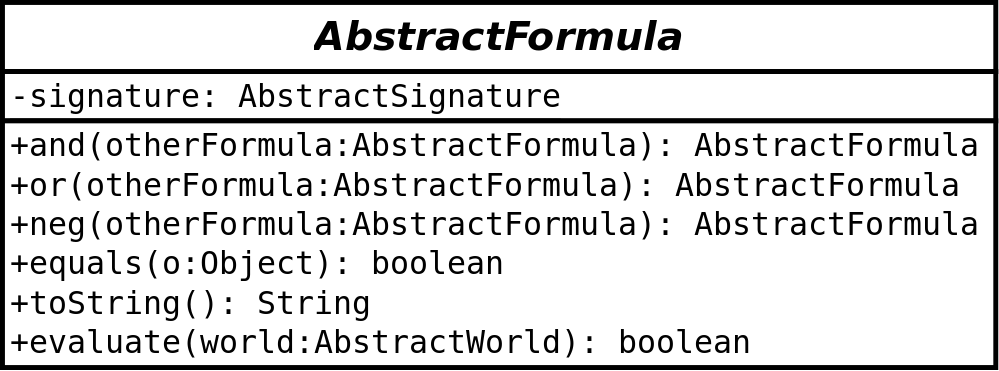
\includegraphics[width=0.55\linewidth]{bilder/AbstractFormula.png}
\caption{Klassendiagramm AbstractFormula}
\label{pic:abstractformula}
\end{figure}


Die grundlegende Klasse der Aussagenlogik ist die abstrakte Klasse AbstractFormula, welche in \autoref{pic:abstractformula} als Klassendiagramm dargestellt wird. Alle Aussagen basieren auf dieser Klasse und entsprechend erben alle konkreten Objekte von dieser. Sie stellt die so Schnittstelle für die konkreten Implementierungen dar und bietet auch selbst einige Funktionen. Die einzige Variable ist die gewählte Signatur \textit{signature} in Form einer Instanz von AbstractSignature als statisches Objekt für alle Instanzen von erbenden Objekten. Weiterhin besitzt die Klasse 6 Methoden, von denen 4 konkret implementiert und 2 abstrakt sind. Implementiert ist zum einen die Methode \textit{and(AbstractFormula otherFormula)}, sie gibt einfach ein Objekt \textit{Conjunction} zurück welches eine Konjunktion aus dem aktuellen (this) Objekt und dem übergebenen ist. Überschrieben wird diese Methode nur in der Klasse Conjunction. Analog dazu verhält sich die Methode \textit{or(AbstractFormula otherFormua)}, welche ein Object der Klasse \textit{Disjunction} zurückgibt. Diese Methode wird ausschließlich von der Klasse \textit{Disjunction} überschrieben. Die dritte konkret Implementierte Methode ist die Negation, aufrufbar mit \textit{neg()} ohne Parameter. Diese Methode gibt eine Negation in Form von \textit{new Negation(this)} zurück. Überschrieben wird diese Methode nur im der Klasse \textit{Negation} selbst. Die letzte konkrete Methode der Klasse \textit{AbstractFormula} ist die Methode \textit{equals(Object o)}, die in \autoref{code:equals-pconditional} abgebildet ist. Sie ist als \textit{final} deklariert und wird demzufolge von keiner erbenden Klasse überschrieben. Wie im Code zu sehen, überprüft die Methode zuerst, ob das übergebene Objekt eine Instanz der Klasse \textit{AbstractFormula} darstellt. Dann wird für alle möglichen Welten der Signatur geprüft, ob die Evaluierung der Welt des übergebenen Objekts das gleiche Ergebnis zurückgibt wie die Evaluierung des aktuellen Objekts (this). Ist das einmal nicht der Fall, wird sofort false zurückgegeben. Wenn die Evaluierung für alle möglichen Welten das gleiche Ergebnis zurückgibt, sind die beiden Objekte gleich im Sinne der \textit{equals(..)} Methode. \\
Weiterhin existieren die abstrakten Methoden \textit{evaluate(World world)} und \textit{toString()}, die jeweils von allen erbenden Klassen überschrieben werden.


\begin{figure}
\begin{lstlisting}
public final boolean equals(Object o) {
    if (!(o instanceof AbstractFormula))
        return false;
    for (AbstractWorld world : signature.getPossibleWorlds()) {
        if (!this.evaluate(world) == ((AbstractFormula) o).evaluate(world))
            return false;
    }
    return true;
}
\end{lstlisting}
\caption{\textit{equals(Object o)} Methode der Klasse AbsractFormula}
\label{code:equals-pconditional}
\end{figure} 



\subsubsection{Atom}


Die Klasse Atom repräsentiert einfach ein einzelnes Atom als Aussage und erbt vonAbstractFormula. Ein Objekt dieser Klasse besitzt eine Instanzvariable mit dem Namen \textit{variable} des Typs \textit{Var}, die den Wert $a$, $b$ oder $c$ annehmen kann. Die \textit{evaluate(AbstractWorld world)} Methode funktioniert folgendermaßen: Sie schaut auf den Variablennamen der in \textit{variable} gespeichert ist und vergleicht diesen mit dem Wert dieser Variable in der übergebenen AbstractWorld und gibt dann zurück ob die Variable in der AbstractWorld true oder false ist. Die zweite Methode der Klasse Atom überschreibt die \textit{toString()} Methode und gibt einfach den Namen der \textit{variable} als String zurück. Die \textit{toString()} Methoden von komplexeren Aussagen als Atom setzten sich dann aus deren Teilaussagen zusammen und rufen so letztendlich auch die \textit{toString()} Methode der Atome auf.


\subsubsection{Conjunction}
Die Klasse \textit{Conjunction} repräsentiert eine Konjunktion aus einer Menge von AbstractFormulas. Diese werden in einer ArrayList<AbstractFormula> gespeichert. Instanzen der Klasse können auf zwei mögliche Arten gebildet werden: Einerseits direkt per Konstruktor in Form von \textit{new Conjunction(AbstractFormula...formulas)} oder andererseits indem auf einer Instanz von AbstractFormula die Methode \textit{and(AbstractFormula formula)} aufgerufen wird. Dabei ist die Klasse \textit{Conjunction} die einzige AsbstractFormula Implementierung, welche die \textit{and(..)} Methode überschreibt. Sie erstellt im Gegensatz zu allen anderen eine neue Conjunction mit einer Liste die aus der FormulaList der aktuellen (this) Conjunction und der hinzugefügten Conjunction besteht. Dadurch stehen alle Elemente der bisherigen \textit{Conjunction} und der hinzugefügten AbstractFormula gleichberechtigt nebeneinander in der FormulaList. Ohne die Überschreibung würde eine \textit{Conjunction} mit einer \textit{Conjunction} als Element entstehen, was zwar korrekt wäre, aber unnötig verschachtelt und in der Darstellung schwerer zu lesen. Bildlich gesprochen werden so einfach die Klammern des Terms aufgelöst. Die \textit{toString()} Methode reiht einfach die Elemente der FormulaList ohne spezielles Zeichen dazwischen zur Verbindung aneinander, entspricht so der verkürzenden Darstellung aus \cite{beierle19}. Die \textit{evaluate(AbstractWorld world)} Methode der Klasse Conjunction evaluiert die einzelnen Teilaussagen aus der FormulaList und gibt falsch zurück sobald ein Element der FormulaList falsch ist. Das entspricht einer lazy evaluation und spart unnötige Rechenoperationen. Erst wenn alle Elemente der FormulaList true zurückgeben gibt auch die \textit{Conjunction} insgesamt true zurück.


\subsubsection{Disjunction}


Die Klasse \textit{Disjunction} repräsentiert eine Disjunktion und ist analog zur gerade beschriebenen Klasse Conjunction aufgebaut. Sie beinhaltet eine ArrayList<AbstractFormula> formulaList in der die Elemente der Konjuntion gespeichert sind. Ebenfalls ist sie per Konstruktor als \textit{new Conjunction(AbstractFormula...formulas)}  mit einem Array instanziierbar. Die Methode der Klasse AbstractFormula \textit{or(AbstractFormula formula)} wird als einzige durch die Klasse \textit{Disjunction} überschrieben und erstellt hier eine neue Conjunction mit einer Liste aus den Elementen der Ursprünglichen Conjunction und dem hinzugefügten Element anstatt einer verschachtelten Conjunction. Die \textit{toString()} Methode der Klasse Conjunction gibt die Elemente als String mit einem Komma getrennt aus, um die Konjunktion von der Disjunktion besser zu unterscheiden. So wird die Konjunktion aus $a$ und $b$ als $ab$ und die Disjunktion aus den beiden Variablen als $a,b$ dargestellt. Die dritte Methode der Klasse \textit{Disjunction} überschreibt die \textit{evaluate(World world)} Methode der Klasse AbstractFormula. Hier findet ebenfalls eine lazy evaluation statt: Die Methode gibt true zurück sobald ein Teilausdruck der formulaList true ist und gibt false zurück wenn alle Teilausdrücke false zurückgeben.


\subsubsection{Negation}


Negation ist die letzte hier beschriebene Implementierung von AbstractFormula. Das einzige Attribut der Klasse ist die \textit{AbstractFormula} formula, also der Term der negiert wird. Die Klasse ist eine Art Wrapper für die beinhaltete \textit{AbstractFormula}. Ein Objekt kann wieder zum einen direkt per Konstruktor als \textit{new Negation(AbstractFormula formula)} erzeugt werden. Die andere Variante ist das aufrufen der \textit{neg()} Methode auf einer Instanz von \textit{AsbstractFormula}. Die \textit{neg()} Methode der Klasse \textit{AsbstractFormula} wird hier überschrieben und gibt die AbstractFormula zurück. Das Vermeidet das Erstellen einer Negation von einer Negation eines Terms, was zwar korrekt aber unnötig kompliziert wäre. Die \textit{toString()} Methode gibt die eingeschlossene \textit{AbstractFormula} mit vorangestelltem "!" wieder. Falls die \textit{AbstractFormula} dabei keine Instanz von Atom ist wird die \textit{AbstractFromula} dabei von Klammern eingeschlossen, um sie eindeutig interpretierbar zu machen. Die \textit{evaluate} Methode gibt einfach die Umkehrung (Java: "!") der eingeschlossenen \textit{AbstractFormula} wieder.


\subsection{Die Klasse PConditional}


\begin{figure}
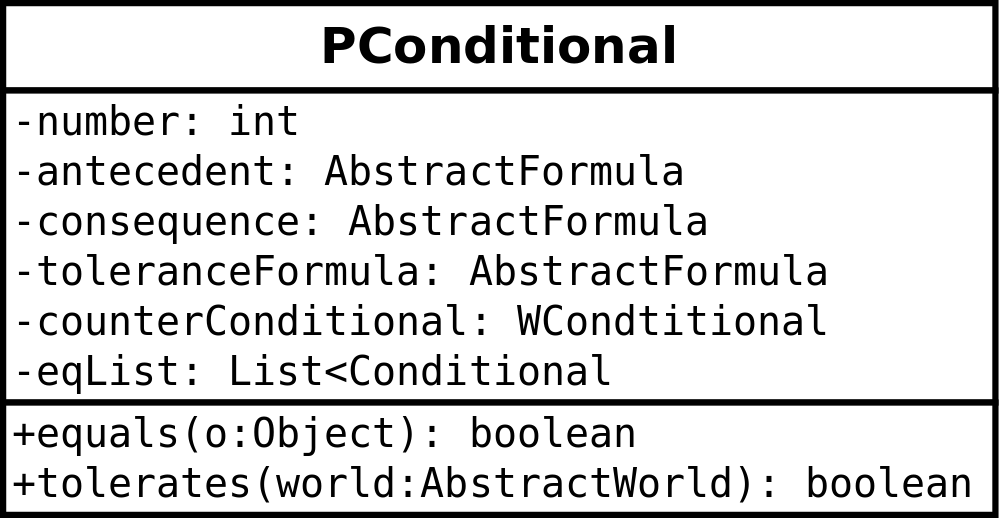
\includegraphics[width=0.45\linewidth]{bilder/PConditional.png}
\caption{PConditional}
\label{pic:pconditional}
\end{figure}


Die Klasse PConditional repräsentiert ein Konditional und unterstützt im Gegensatz zur Klasse WConditional die Verarbeitung mit Aussagenlogik. Ein vereinfachtes Klassendiagramm von PConditional ist in \autoref{pic:pconditional} zu sehen. Die meisten Attribute werden bei der Übersetzung von WConditional zu PConditional übernommen. Wie genau diese Übersetzung abläuft, ist in \autoref{sec:übersetzung} beschrieben. Als Attribute besitzt die Klasse ein Antecedent und Consequence jeweils in Form einer AbstractFormula, wie unter \autoref{sec:logic} beschrieben. Die Referenz toleranceFormula als AbstractFormula wird direkt bei der Konstruktion des Objekts einmalig erstellt. Sie wird nach \autoref{def:toleranz} für ein Konditional $B|A$ in der Form $\overline{A} \vee B$ in einer AbstractFormula gebildet, konkret als Code  $toleranceFormula = antecedent.neg().or(consequence)$. Die toleranceFormula wird in einer Instanzvariable zwischengespeichert und nicht bei jedem Test   auf Toleranz neu erzeugt, da der Test sehr oft aufgerufen wird und so etwas Rechenzeit eingespart wird. Die dazugehörige Methode \textit{boolean tolerates(world: AbstractWorld)} besteht aus der einen Zeile \textit{return toleranceFormula.evaluate(world)}. Die equals(Object o) Methode ist so implementiert, dass sie true zurückgibt, wenn das übergebene Objekt ein PConditional mit derselben Nummer ist. Einfach die Nummer der Konditionale zu verwenden ist hier die simpelste Variante, ein Vergleich von Antecedent und Consequence wäre auch naheliegend. Die Entscheidung, nur die Nummer zu vergleichen, beruht auf ihrer Einfachheit. Zuverlässig ist sie trotzdem, da die Konditionale nur an einem einzigen Punkt im Programm erstellt werden und die Nummer direkt im Konstruktor mit Antecedent und Consequence gesetzt wird.


\subsection{Übersetzung der Konditionale}
\label{sec:übersetzung}
In diesem Abschnitt wird beschrieben, wie die Konditionale aus der Form als Instanzen von WConditional als Instanzen von PConditional übertragen werden. Genauer gesagt, der interessante Teil ist es Antecedent und Consequence jeweils aus der Form WorldsList in die Form AbstractFormula zu bringen. \\
Dabei sind zwei grundsätzliche Vorgehensweisen vorstellbar: Zum ersten der Ansatz, der im Folgenden als \textit{nativer} Ansatz benannt wird: Die Liste der möglichen Welten wird einfach als Disjunktion von Konjunktionen aufgefasst. Als Beispiel, unter Signatur $\Sigma=\{ab\}$ ist sei Liste Möglicher Welten $ab, !ab$. Dann ist der aussagenlogische Term dafür $(a \wedge b) \vee (\overline{a}\wedge b)$. Die zweite Variante für die Übersetzung ist, den kürzesten möglichen Term zu suchen. Im genannten Beispiel ist das $a$. Allerdings ist die zweite Variante
\\
todo: translator beschreiben

todo:Performance Vergleich mit kurzen Übersetzungen als Begründung warum die nicht verwendet werden.
\subsection{Wissensbasen}
Beschreibung der Klasse KnowledgeBase. Klassendiagramm.
beschreiben, warum numbers kb gelöscht wurde (bringt nix. spart nicht viel speicher ist aber deutlich langsamer)


\section{Zwischenspeicherung der Daten}
In diesem Abschnitt wird beschrieben, wie die Arbeitsdaten von GenKB verwaltetund gespeichert werden. Während einer Iteration k von GenKB werden dabei Daten aus Iteration $ k - 1$ verarbeitet und neue Daten unter $k$ selbst abgelegt. Dadurch entstehen große Mengen von Daten, welche bis zur jeweils nächsten Iteration behalten werden müssen. Dabei stellt sich schnell heraus, dass es für den Erfolg des ganzen Programms kritisch ist, diese Daten so effizient und sparsam wie möglich zu verwalten. \\
Einzelne Datensätze werden dabei als Objekte gespeichert, welche jeweils eine Wissensbasis und eine Menge an Kandidaten enthalten. Die Verwaltung dieser Datensätze übernimmt ein Puffer, der die Daten Wahlweise entweder im Arbeitsspeicher oder auf der Festplatte speichert und zur Verfügung stellt. 

\subsection{Paare aus Wissensbasis und Kandidaten}
In diesem Abschnitt werden die Paare aus Wissensbasen und Kandidaten, um welche die Wissensbasis erweitert werden kann, beschrieben. Als Paare wird hier die Einheit aus Wissensbasis und Menge an Kandidaten bezeichnet, welche im Algorithmus GenKB in \cite{beierle19} in Zeile 5 initialisiert und in Zeile 8ff bearbeitet wird. Dargestellt wird diese Einheit als mit charakteristischen dreieckigen Klammern in der Form $<R, C>$, was auch hier so beibehalten wird. \\
Im Programm werden die zwei Implementierungen genutzt, die hier vorgestellt werden. Beide erben von \textit{AbstractPair}, was die einige Gemeinsamkeiten beider Klassen vereint und hauptsächlich die Schnittstelle der Paare bildet. Die beiden Implementierungen unterscheiden sich hauptsächlich in der Speicherung der Kandidaten, da davon sehr viele verwaltet werden müssen. Die erste Implementierung ist RealPair, hier werden die Kandidaten als Liste von Konditionalen verwaltet. Das ist naheliegend, einfach und schnell, benötigt aber sehr viel Arbeitsspeicher. Die zweite Option CompressedPair komprimiert die Liste der Kandidaten und spart dadurch viel Arbeitsspeicher, ist dafür jedoch langsamer. Deswegen wird im Programm die Version RealPair benutzt, wenn die Daten sowieso auf der Festplatte zwischengespeichert werden und die Option CompressedPair wird genutzt wenn die Daten im Arbeitsspeicher gehalten werden sollen.

%todo: clear methoden erklären
\subsubsection{Abstract Pair}
\label{sec:abstractpair}

\begin{figure}
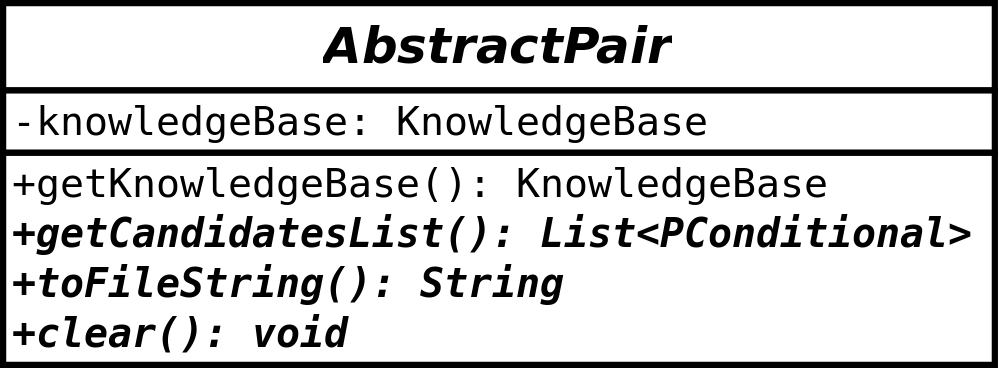
\includegraphics[width=0.45\linewidth]{bilder/AbstractPair.png}
\caption{AbstractPair}
\label{pic:abstractpair}
\end{figure}



Wie beschrieben, vereint die Klasse AbstractPair die Gemeinsamkeiten ihrer beiden Implementierungen und bildet die Schnittstelle für deren Verwendung, entsprechend ist die Klasse selbst eher übersichtlich. Ein etwas vereinfachtes Diagramm der Klasse AbstractPair ist in \autoref{pic:abstractpair} zu sehen. Als Attribut besitzt die Klasse nur die Wissensbasis in Form eines KnowledgeBase Objekts und eine Map<int,WConditional> in der alle Konditionale von NFC unter ihrer Nummer abgespeichert sind. Des weiteren besitzt die Klasse 3 abstrakte und eine konkrete Methode. Die Methoden \textit{getKnowledgeBase()} und \textit{ getCandidatesList()} sind selbsterklärend. Die \textit{toFileString()} Methode gibt einen String zurück der die Klasse in einen String transformiert um diesen auf der Festplatte zu speichern. Die letzte Methode \textit{clear()} ist dazu da Speicher zu sparen und löscht die Daten in der Klasse, wenn diese nicht mehr gebraucht werden. Die Implementierungen von AbstractPair unterscheiden sich besonders darin, wie sie die Liste der Kandidaten speichern.

\subsubsection{Real Pair}
Die Klasse \textit{RealPair} speichert die Liste der Kandidaten zur Erweiterung der enthaltenen Wissensbasis als List<PConditional>. Das ist naheliegend und in der Verarbeitung schnell, benötigt jedoch sehr viel Speicher. Deshalb wird die Klasse RealPair nur in Verbindung mit Speicherung der Daten auf der Festplatte genutzt. Dadurch existieren zu jedem Zeitpunkt nur recht wenige Objekte dieser Klasse. Der hohe Speicherbedarf ist dann unproblematisch und die hohe Verarbeitungsgeschwindigkeit kann genutzt werden. \\
Die Kandidaten werden einfach als ArrayList<PConditional> gespeichert. Ein einfacher Konstruktor in Form von \textit{RealPair(KnowledgeBase knowledgeBase, List<PConditional> candidates)} steht bereit, um das Paar in GenKB in Zeile 5 und 12 zu erstellen. Die eigentliche Komplexität in der Klasse RealPair liegt darin, alle Informationen der Klasse in einen möglichst kurzgefassten String umzuwandeln, um die Klasse auf der Festplatte zu speichern und analog dazu die Klasse aus diesem Stück Text wieder zu rekonstruieren.




\begin{figure}
\begin{lstlisting}
KB
1{1}
C
3-6050
END
\end{lstlisting}
\caption{\textit{RealPair} als String zum Speichern auf der Festplatte}
\label{code:pair-text}
\end{figure} 


In \autoref{code:pair-text} ist die Repräsentation des ersten RealPairs mit der Signatur $\Sigma=\{abc\}$  als Text abgebildet, eine Erklärung davon folgt sofort. In Zeile 1 ist mit KB einfach die Information kodiert, dass als nächstes die KnowledgeBase beschrieben wird. Die Beschreibung der Wissensbasis in Zeile 2 zeigt als erstes die Nummer vor der Klammer, die die Nummer der Wissensbasis bezeichnet, hier die 1. Innerhalb der geschweiften Klammern befinden sich die Nummern der Konditionale der Wissensbasis, hier ebenfalls die 1. Das C in Zeile 3 kündigt an, dass die Liste der Kandidaten folgt. In Zeile 4 dann die komprimierte Liste der Kandidaten, die etwas erklärungsbedürftig ist. Sie wird hier so interpretiert, dass alle Konditionale mit den Nummern 3-6050 in die Liste der Kandidaten aufgenommen werden sollen. Das dafür werden die Konditionale aus der Map<int, WConditional> aus AbstractPair abgerufen. Das ist in diesem Beispiel sehr einfach, da sich in der Menge keine Lücken befinden. Wenn sich Lücken darin befinden, werden die einzelnen zusammenhängenden Bereiche von Kommas getrennt. Beispielsweise bedeutet "3-5, 7-6050" dass alle Konditionale außer den Nummern 1,2 und 6 in die Liste der Kandidaten aufgenommen werden sollen. Hier wird offensichtlich, dass die Effizienz dieser Speicherung dann besonders hoch ist, wenn kaum Lücken vorhanden sind. Das ist in GenKB bei niedrigen Werten für k der Fall. Mit steigendem k steigt auch die Menge der Lücken und damit der Speicherbedarf für das RealPair. Da jedoch aufgrund der Geschwindigkeit sowieso nur geringe Werte von k relevant sind, ist damit eine sehr effiziente Speicherung der RealPairs sichergestellt. In Zeile 5 des Beispiels hat der Eintrag END die Bedeutung, dass das Paar hier endet. Dadurch werden die verschiedenen Paare innerhalb einer Datei voneinander getrennt. Da während des Programmablaufs sehr viele Paare erstellt werden, wäre es ineffizient, für jedes Paar eine eigene Datei zu erstellen. Das Schreiben der einzelnen Dateien auf die Festplatte wäre dann der Flaschenhals für die Geschwindigkeit. Deshalb werden sehr viele Paare in eine einzelne Datei zusammengefasst. Als guter Wert für die Menge der RealPairs pro Datei ist die Entscheidung nach einigem Testen auf 2000 gefallen, der genaue Wert ist jedoch für den Programmablauf unwichtig. \\
Um ein Objekt in die Form für die Textdatei zu bringen, besitzt es eine Methode \textit{toFileString()} die eben genau diesen String erzeugt. Analog dazu besitzt die Klasse RealPair auch einen Konstruktor \textit{RealPair(String string)}, der ein Objekt der Klasse aus einem solchen String erzeugen kann. Diese Methoden sind recht umfangreich und aber keine überraschenden Funktionen, deshalb sind sie hier nicht weiter erklärt.



\subsubsection{Compressed Pair}
Die Klasse  \textit{CompressedPair} ist die Implementierung von AbstractPair, die verwendet wird, wenn die Daten nicht auf der Festplatte zwischengespeichert werden sondern im Arbeitsspeicher verbleiben. Wie der Name schon verrät, ist dafür ein Kompressionsmechanismus eingebaut. Dieser betrifft wie bei der Speicherung der RealPairs die Liste der Kandidaten. Ähnlich wie bei der Speicherung in RealPair werden zusammenhängende Nummern von Konditionalen genutzt, um Speicherplatz zu sparen. Dazu besitzt die Klasse CompressedPair ein Array von zweidimensionalen Arrays von Integer Werten. Damit werden die Daten im Arbeitsspeicher abgelegt. Die Wahl des Datentyps fällt auf Arrays statt Listen, da die Speicherung hier viel effizienter erfolgen kann. In Java existiert der simple Datentyp int und analog dazu die Möglichkeit Integer Werte als Objekte der \textit{Integer} Klasse zu speichern. Der simple int Typ benötigt dabei jedoch deutlich weniger Speicher als der Overhead eines Objekts der Klasse Integer. Listen können in Java jedoch nur von Integer Objekten erstellt werden, nicht von simplen int Werten, daher müssen die Werte hier in Arrays gespeichert werden.\\
Der Kompressionsalgorithmus sucht wieder zusammenhängende Mengen von Konditionalen im Format (Nummer des ersten Konditionals) (Nummer des letzten Konditionals). Diese werden als int Array mit der Länge zwei abgelegt. Von diesen int Arrays der Länge zwei wird dann ein wiederum Array erstellt und darin die gesamte Menge der Konditionale gespeichert. Die Größe des gesamten Arrays beträgt dann [Menge der zusammenhängenden Bereiche][2]. Solange die zusammenhängenden Bereiche groß sind, funktioniert die Kompression sehr gut. Mit steigendem Wert von k kommen jedoch immer mehr Lücken hinzu und die Speicherung wird zunehmend umständlich. \\
Mit der Signatur $\Sigma=\{abc\}$ werden nur geringe Werte für k erreicht, demzufolge ist die Speicherung sehr effizient. Mit der Signatur $\Sigma=\{ab\}$ werden jedoch höhere Werte für k erreicht. Zusätzlich ist hier die Menge der Kandidaten viel geringer, sodass diese Kompression kaum Vorteile bringt. Das ergibt dann den folgenden Effekt: Für geringe Werte für k wird weniger Speicher benötigt, für hohe Werte für k wird sogar mehr Speicher benötigt. Da die Signatur  $\Sigma=\{abc\}$ im Vordergrund steht wird die Ineffizienz für $\Sigma=\{ab\}$  jedoch ignoriert.\\
Der Konstruktor der Klasse CompressedPair ist in der Form \textit{CompressedPair(KnowledgeBase knowledgeBase, List<PConditional> candidates)},  ein Erstellen aus Textdateien entfällt. Die beschriebene Komprimierung erfolgt direkt im Konstruktor. Wenn die Liste der Kandidaten mit \textit{getCandidatesList()} abgerufen wird, wird die List<WConditonal> aus dem komprimierten int Array erstellt. Da dieser Vorgang recht kompliziert ist, dauert das aufrufen der Methode \textit{getCandidatesList()} deutlich länger als bei Objekten von RealPair. Der Konstruktor ist ebenfalls deutlich zeitintensiver als RealPair, jedoch entfällt bei CompressedPair das eher langsame Lesen und Schreiben auf der Festplatte dafür komplett.



%todo: vlt deutsche namen anstatt klassennamen?
\subsection{Pair Buffer}
\label{sec:pairbuffer}


Als \textit{PairBuffer} wird die Datenstruktur bezeichnet, welche die Menge der im Abschnitt zuvor beschriebenen Paare aus Wissensbasis und Kandidaten verwaltet und speichert. Dabei sind zwei verschieden Varianten implementiert: eine Variante legt die Daten im Arbeitsspeicher ab während die andere Variante die Festplatte nutzt. Der Nutzer kann in der grafischen Oberfläche in den Optionen unter "Buffering" wählen, ob die Daten auf der Festplatte gespeichert werden sollen oder ob der Arbeitsspeicher verwendet werden soll.


\subsubsection{AbstractPairBuffer}
Die Klasse \textit{AbstractPairBuffer} ist die Abstrakte Klasse die von beiden Varianten der Speicherverwaltung implementiert wird und hat hauptsächlich den Charakter eine Schnittstelle. Da sich die Implementierungen stark unterscheiden, stellt diese Klasse selbst keine eigene Funktionalität bereit. Die abstrakten Methoden der Klasse lassen sich in die folgenden Kategorien einteilen:

\begin{itemize}

\item{Starten und Beenden von Iterationen}
\item{Hinzufügen und Abrufen von Datensätzen}
\item{Abrufen Statusinformationen zum Anzeigen in der grafischen Oberfläche}
\end{itemize}


%todo: reread and good language
\subsubsection{RamPairBuffer}
Die Klasse  RamPairBuffer ist einfach aufgebaut, sie ist im Prinzip eine Container für eine passive Datenstruktur. Die Klasse besitzt keine eigenen Threads sondern nur das Objekt zur Aufnahme der Daten und Methoden, um diese zu verwalten. Die Daten werde in einer List<List<AbstractPair>> gespeichert, die folgendermaßen aufgebaut ist: Die äußere Liste beinhaltet Listen von Datensätzen in Form von AbstractPair, konkret werden hier nur CompressedPair Objekte gespeichert. Für jede Iteration wird der äußeren Liste ein neues Element hinzugefügt, der Index entspricht hier der Iterationsnummer $k$ von GenKB. \\
Wenn also eine Iteration $k$ beginnt, wird entsprechend für das Element $k$ eine neue ArrrayList<AsbtractPair> in die äußere Liste eingefügt. In diese Liste werden während der Iteration $k$ die Daten abgelegt, die Daten aus $k-1$ werden zur Verarbeitung nach und nach abgerufen. Während des Abrufens werden bereits die nicht mehr benötigten Elemente größtenteils gelöscht, das geschieht durch die unter \autoref{sec:abstractpair} beschriebene \textit{clear()} Funktion der Pairs. Dadurch wird der Speicherbedarf einer Iteration deutlich verringert. Gleichzeitig wird mit dem Anlegen der neuen Liste für $k$ die Liste $k-2$, sofern diese vorhanden ist, vollständig gelöscht, denn sie wird dann  nicht mehr gebraucht.

\subsubsection{HDDPairBuffer}




\section{Berechnung der Wissensbasen}
logische reihenfolge finden.



Hier ein schönes Übersichtsdiagramm. Hier auch was zum Threading.


\subsection{Implementierung von GenKB}
Erstmal Simple Creator. Funktioniert Parallel? Das wär gut, auch zum gegenüberstellen.
\subsection{KnowledgeBase Writer}
beschreiben. dummy writer und writer. Parallel Writer?

\subsection{Beschreibung der grafischen Oberfläche}
möglicherweise auch am anfang analog zu kb creator? würde die schritte vereinfachen! \\
auf jeden fall linke und rechte seite trennen.
\subsection{Betrachtung von Knowledge Base Creator mit JVisualVM}
kurz was zum programm mit link \\
eventuell auch als eigener punkt damit das hier nicht zu viel wird. screenshots und so. threading beschreiben. rechenzeit pro methode betrachten? speicher betrachten?



\newpage

\bibliography{lit} 
\end{document}